% !TEX root = ./english.tex

\chapter{Common Module - Rosemary Dobson Poetry}

\section{Young Girl at a Window} \label{1/11/2024}
	\subsection{Stanza 1}
		\begin{itemize}
			\item Title - The poem's simple title evokes the museum label of a pictorial artwork
			\item Second person - Speaker is speaking to someone else, therefore standing side by side as observer of the girl. "omnipresent"
			\item Liminal space between childhood and adulthood
			\item Poem creates a juxtaposition of movement and standing still
				\subitem dichotomy between static nature of an artwork
			\item "Lift you hand to the window latch" - "Lift" and "turn" are commands. Imperative language instructs, creating the impression that the speaker is directly addressing the subject, second person also immerses audience and may imply direction of instructions to the reader. Collective experience of coming of age
			\item Position at a window - Crossing a threshold, metaphorical setting that is familiar. Shows the liminal state between inside and outside. Room represents the security and safety of being a child, also stifling, restrictive
			\item Looking at the horizon represents looking into the future (outside)
			\item Diction (word choice) "sigh" connotes a sense of wistful unease, as the girl contemplates taking action, but ends up resigning herself. Shows conflicted state of mind, associated with liminal state
			\item Metre - Second line of the first stanza "Sighing, turn and move away" catalectic (shortened by one syllable) Mimics incompleteness, irresolute gesture
			\item "More than mortal swords are crossed / On thresholds at the end of day" - Allusion to the Christian myth of Eden, supernatural forces were positioned at the gates of paradise - Angle outside with flaming sword, irreversibility of time and the fact that we cannot return to childhood "threshold" implies the transition between states - metaphor of sensing the end of childhood
			\item "The fading air is stained with red" - Red sky, sunset - connotations of the word stained, red also associated with blood, war, violence. Dictional word choices that evoke battle. Also may represent menstruation
			\item "Since Time was killed and now lies dead" - Personification of time, capital letter - In Greek myths, father of Time or Kronos was similarly personified, ate children, symbolic of time's relentless consuming nature - Killing time is a common idiom - To do something frivolous to pass an hour or so while waiting for something to happen. Dobson extends this idiom, making it more literal. A restless anticipation of the future, feeling that time has stopped, frozen in a single moment
		\end{itemize}

	\subsection{Stanza 2}
		\begin{itemize}
			\item "Or Time was lost." Time is personified, questioning the relationship between the stillness of the poem and the unceasing flow of time
			\item First line employs strong medial caesura (pause in the middle of a line marked by a full stop) - Creates suspense, breaks the smooth momentum of the poem
			\item "But someone saw / Though nobody spoke and nobody will" - "someone" is ambiguous, could be the painter who turned the girl's experience into a representation
			\item "While in the clock against the wall / The guiltless minute hand is still" - The minute hand is a synecdoche for the clock and time as a whole (using a part to represent the whole) - metaphor for the innocence of the passing of time,maintains narrative of indecision, The inherent stasis of a painting is used as a metaphor for the intensity and suspense of the girl's awareness that she stands at a crossroads in her life, which creates a sense that time is standing still - Clock doesn't tick - inaction
			\item "The watchful room, the breathless light / Be hosts to you this final night" - Nouns without verbs, connoting suspense of normal actions, juxtaposes the word "final" which implies that change must come
		\end{itemize}

	\subsection{Stanza 3}
		\begin{itemize}
			\item "Over the gently-turning hills / Travel a journey with your eyes" - Movement is restored, imperative tone returns, implying a new sense of purpose and direction, high modality
			\item "Travel a journey with your eyes / In forward footsteps, chance assault-" - The fricative alliteration ("v" and "f" create an airy, breathless sound) reinforce the newfound sense of momentum and purpose
			\item "This way the map of living lies." - If the girl is imagined looking out of the picture frame, then "this way" is out of the pictorial frame into the real world. Is there a point here about art and life, that representations might compensate, but not substitute living it
		\end{itemize}

	\subsection{Example Question} \label{(cont.) 6/11/2024}
		\textbf{How does Dobson's poetry explore the human experience of transience? Write one paragraph (approx. 250 words)}

		All human experiences are embedded in time; our awareness of temporality reveals\dots
		\begin{enumerate}
			\item Topic sentence - All human experiences are embedded in time; our awareness of temporality reveals\dots
			\item Introduce the text and thesis statement - Rosemary Dobson's (1943) ekphrastic (introspective, lyrical) poem \underline{Young Girl at a Window} is a subtle exploration of the inescapably transient nature of the human experience, examining how the transition between stages of life can be daunting (ambivalent, confronting, etc.)
			\item Chronologically analyse textual evidence (min. 6 small quotes)
				\subitem Embed maximum devices and quotes into sentences; Layered sentences; Link back to the question
			\item Concluding sentence - Come outside the world of the text, link to the broader human experience. Use words of the rubric, eg. individual, collective, ignite, challenge, anomalies, paradox, assumptions, power of storytelling
		\end{enumerate}

	Dobson explores the transience and temporality of the human experience by capturing the fleeting aspects of a singular point in time in her ekphrastic poem "Young Girl at a Window". The title is comparable to that of a pictorial artwork, inviting its audience to reflect on the poem as a representation of both literature and art. By doing so, Dobson outlines the limited nature of art forms in general, portraying one point of the ongoing human experience. This concept is further extended as a metaphor for human life as a temporary and fleeting occurrence in the grand scheme of nature. The speaker directs its subject to "Lift" and "turn", establishing an imperative tone that suggests an inferiority of the girl. This assertive and calm tone contrasts the violent and confrontational imagery of "air \dots stained with red" and "Time \dots killed and now lies dead." This contrast creates a sense of the unimportance of the individual experience in comparison to the whole of time. The second stanza begins with a strong medial caesura, breaking the even rhythm of the first stanza. The tension created is used to analyse both the shortness of both one human experience, as well as the life of an individual. The "guiltless" minute hand "is still", yet time continues to progress.

\section{Over the Hills} \label{6/11/2024}
	This workman dredges home at dusk \\
	With bluntly forward boots that toss \\
	The roan earth out like chaff behind; \\
	His swung cap scooping cups of wind, \\
	He crests the hill and fills the sky, \\
	His eyes' lit windows facing west \\
	To take the lemon-coloured light \\
	While the day slowly drains away, \\
	Or strides from hill to hill and strikes \\
	A match against the friendly stars \\
	(Hanging his cap on the horn of the moon). \\
	Now as he stands to light his pipe \\
	With quite unconscious insolence, \\
	He could move mountains if he cared, \\
	But a mountain in the palm of one's hand \\
	Is a troublesome thing, so he lets them lie— \\
	Or lifts one, looks at it, quiets the trees, \\
	Turns it slowly and puts it down.

\section{Summer's End: After the Summer Season} \label{13/11/2024}
	\subsection{Structure}
		One stanza with 17 lines

		Free verse:
		\begin{itemize}
			\item Non-metrical (not written in metre), non-rhyming lines that follow the natural rhythm of speech. A regular pattern may form, but not adhere to a metrical plan
			\item Free verse emphasises the longing for creative freedom and tension in how the domestic sphere inhibits the broader creative wilderness the poet wishes to inhabit.
		\end{itemize}

		Punctuation
		\begin{itemize}
			\item The colon in "Who married a mortal: who weeps at the edge of the water" creates a boundary that cannot be crossed
		\end{itemize}

		Biblical allusion:

			\subitem The poem features a range of bestial imagery (seagulls, flies, cat). The language employs grand biblical allusions to “miraculous cleansing … waters” and the overwhelming emotional landscape of floods. These emotional undercurrents juxtapose with the frivolity of “sun-hats” and “surfboards” to imply an insular and inexpressible grief. At the same time, the images employed of the sleekly prowling cat hints at recovery and repose. The backdrop of a beach at the end of summer is uniquely Australian, depicting nature as both a place of destruction and unwavering solace. This exemplifies the 

		Alliteration/repetition:
		\begin{itemize}
			\item “where, who, who, where”.
			\item The use of alliteration suggests that the human experience is perpetuated through questions
		\end{itemize}
		
		Appropriation and Intertextuality:
		\begin{itemize}
			\item The appropriation of "The Little Mermaid" by Hans Christian Andersen depicts the archetypal outsider.
			\item Knives symbolise the pain and suffering of the human experience
			\item Despite the pain, the subject is seen to continue her journey regardless of pain and grief
		\end{itemize}
	
		\newpage

	\subsection{Diptychs}
		A diptych (translates to "two-fold") refers to a single artwork with two separate panels joined together. An additional panel would turn it into a triptych.
		\begin{figure}[H]
			\centering
			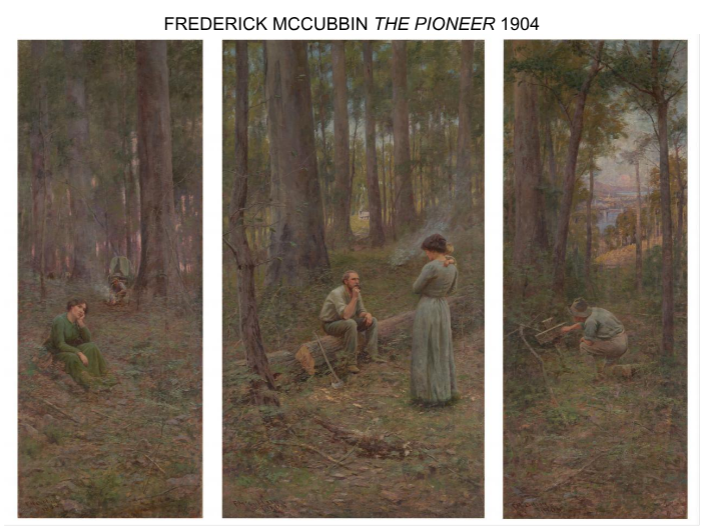
\includegraphics[width=15cm]{diptych example.png}
		\end{figure}

\section{The Conversation Questions} \label{20/11/2024}
	\begin{enumerate}
		\item \textbf{What is the main thematic concern or message of The Conversation?}
		\item \textbf{Discuss one aspect of the poem that is ambiguous. Why is it intentionally so?}
		\item \textbf{Answer the following question in the style of a short answer HSC response:} \\
		\textit{How is the attainment of wisdom essential to the human experience? In your response, refer closely to both Over the Hill and The Conversation. (8 marks)}
		\begin{itemize}
			\item Compare and contrast
			\item Mini-essay structure
		\end{itemize}
		Ideas
		\begin{itemize}
			\item wisdom produces resilience, optimism
			\item connections to nature
			\item unique perspectives
			\item personal wisdom vs. gaining wisdom through connections with people
		\end{itemize}

		\subitem \textbf{Example:} Rosemary Dobson explores how moments of profound simplicity sparks reflection into the world and the self. Whilst Over the Hill portrays wisdom as a quiet and individual experience with the natural world, The Conversation suggests that wisdom is rooted in playful, unspoken exchanges and it is this connection between youth and age that fosters imagination and learning experiences.

		\subitem Topic sentence that outlines the message about wisdom in the first text. Then chronological analysis \\
			Over the Hill captures the experience of solitude for a labourer who embodies wisdom through his harmonious relationship with the natural World

		\subitem Link back to the first text in the paragraph \\
			In contrast, The Conversation presents wisdom as an imaginative and wordless connection between two unlikely interlocuters 
	\end{enumerate}

\section{Amy Caroline} \label{27/11/2024}
	\textbf{Themes}
	\begin{itemize}
		\item Appreciation of age to shape human experience
		\item Importance of memories
		\item Importance of gentility - ie. social superiority demonstrated by politeness and respectability
		\item Valuing experiences across generations
	\end{itemize}

	\textbf{Techniques}
	\begin{itemize}
		\item Free verse - No regular metre or rhyme scheme providing a conversational tone; colloquialised
		\begin{itemize}
			\item Enjambment
			\item Caesura
		\end{itemize}
		\item First person - biographical
		\item Geographical references - "In Bendigo and Eaglehawk"; value of place, associated with memories
	\end{itemize}

	\subsection{Review Questions}
	\begin{enumerate}
		\item What facts does this poem convey regarding the life of Amy Caroline?
		\subitem The poem reveals the selfless and caring aspects of Amy Caroline's life, depicting her nurturing behaviours and how she cares for others. It also describes the hardships that she has experienced and briefly concludes with the regrets that 

		\item How does the poem use paradox to make Amy Caroline relatable? What lessons can be learnt about the human experience through Dobson's depiction of people's lives in \underline{Amy Caroline}?
		\item Write an analytical paragraph using the following topic sentence:
		
		Dobson's (1973) blank-verse poem \underline{Amy Caroline} portrays old age as a time of reconciliation with one's authentic identity;
		
		Dobson challenges the notion of feminine vulnerability, revealing the profound beauty and strength within elderly experiences of femininity.
	\end{enumerate}

\section{Canberra Morning} \label{28/11/2024}
	\textbf{As we \textit{age}, we can \textit{reflect upon} and \textit{view} human experiences. \\
	Discuss this statement with reference to Dobson's \underline{Canberra Morning} and one other poem from the prescribed texts. \\
	In your response, you should compare and contrast how the ideas are explored within the two poems.}

	\begin{itemize}
		\item Highlight or underline key terms of question
		\item Young Girl at a Window - differences in subject matter and perspective. Canberra Morning is about observing others, YGAW is self-contained and looks inward. The speakers in both have age and maturity $\rightarrow$ this allows for reflection. YGAW explores fear of change whilst CM embraces change and the passage of time. Neither positive nor negative.
	\item Summer's End - passage of time, metaphor of different season overlaps both poems
	\end{itemize}

	Human aging brings wisdom built upon experiences that allows people to contemplate and appreciate broader human experiences. Dobson's (1973) anecdotal poems Canberra Morning and \dots

\section{Dobson Essay} \label{13/12/2024}
	Thesis: Temporality and permanent nature of time, shaping individual experience
	How does the poetry of Rosemary Dobson explore the complexities
	Texts:
	\begin{itemize}
		\item Summer's End
		\item Over the Hill
		\item Young Girl at a Window?
	\end{itemize}
	
